\documentclass{article}
\usepackage[utf8]{inputenc}
\usepackage[brazilian]{babel}
\usepackage{url}
\usepackage{graphicx}
\usepackage{geometry}
\usepackage{enumitem}
\usepackage{float}
\usepackage{amsmath}
\usepackage[table,xcdraw]{xcolor}
\usepackage{multirow}
\usepackage{caption}

\geometry{a4paper, left=20mm, right=20mm, top=20mm, bottom=20mm}
 

\begin{document}

\begin{frame}{}
    \hspace*{-0.5cm}
    $\vcenter{\hbox{
\includegraphics[width=1cm]{mackenzie-logo.png}}}$
    $\vcenter{\resizebox{0.95\textwidth}{!}{
        \begin{tabular}{c}
          Leandro N. de Castro \& Daniel Ferrari  \\
          Introdução à Mineração de Dados: Conceitos Básicos, Algoritmos e Aplicações \\
             \hline 
             Marcos Cordeiro de Brito Jr
        \end{tabular}
    }}$
\end{frame}

\begin{center}
  \huge \textbf{CADERNO DE EXERCÍCIOS – PARTE 02} \\ 
\end{center}

\setcounter{section}{4}
\section{CAPÍTULO 05: CLASSIFICAÇÃO DE DADOS}
\subsection{EXERCÍCIOS CONCEITUAIS}
\subsubsection{Durante o desenvolvimento de um modelo de classificação a base de dados é dividida em dois conjuntos. Quais são estes conjuntos e qual é o propósito desta separação}
\textit{Resposta:} Os dois conjuntos são: treinamento e testes. Seu propósito é gerar modelos preditivos capazes de identificar classes ou valores de registros não rotulados com um resultado satisfatório. 

\subsubsection{Discuta por quê para bases de dados reais na maioria das vezes treinar um sistema preditivo até que o erro para os dados de treinamento seja zero não é aconselhável.}
\textit{Resposta:} Durante o processo de treinamento de modelos, mesmo com o desempenho cada vez melhor e a quantidade de erros possa estar decaindo, o desempenho de generalização pode começar a se deteriorar após determinado número de iterações. \\
O ideal é utilizar uma validação cruzada para interromper o treinamento para conseguir obter um melhor resultado.

\subsubsection{O que é a validação cruzada em k-pastas? Qual é a sua finalidade?}
\textit{Resposta:} A validação cruzada em k-pastas consiste em dividir a base de dados em k subconjuntos, sendo k –1 pastas para treinamento e 1 pasta para teste. Esse processo de treinamento e teste é repetido com todos os k subconjuntos, e a média dos desempenhos para as bases de treinamento e as bases de teste é adotada como indicador de qualidade do modelo. \\
A validação cruzada em k-pastas é bastante usual para se estimar o erro de generalização de preditores.


\subsubsection{O que é a matriz de confusão de um problema de classificação binária? Explique os quatro valores apresentados pela matriz.}
\textit{Resposta:} Matriz de confusão é uma forma de apresentar integralmente o desempenho de um algoritmo de classificação binária utilizando uma matriz que relaciona as classes desejadas com as classes preditas. \\
Essa matriz também é conhecida como \textit{matriz de contingência} ou \textit{matriz de erro} e na sua composição ela tem nas linhas os objetos nas classes originais e nas colunas os objetos nas classes preditas.

\begin{center}
  \begin{table}[H]
    \centering
      \begin{tabular}{ll|c|c|}
      \cline{3-4}
                                                                                      &                                                       & \multicolumn{2}{c|}{\cellcolor[HTML]{C0C0C0}Classe predita}         \\ \cline{3-4} 
                                                                                      &                                                       & \cellcolor[HTML]{C0C0C0}Positiva & \cellcolor[HTML]{C0C0C0}Negativa \\ \hline
      \multicolumn{1}{|c|}{\cellcolor[HTML]{C0C0C0}}                                  & \multicolumn{1}{c|}{\cellcolor[HTML]{C0C0C0}Positiva} & VP                               & FN                               \\ \cline{2-4} 
      \multicolumn{1}{|c|}{\multirow{-2}{*}{\cellcolor[HTML]{C0C0C0}Classe original}} & \multicolumn{1}{c|}{\cellcolor[HTML]{C0C0C0}Negativa} & FP                               & VN                               \\ \hline
    \end{tabular}
  \end{table}
\end{center}

Abaixo estão as explicações dos quatro valores apresentados na tabela.

\begin{itemize}
  \item \textbf{VP (verdadeiro positivo):} você previu positivo e é verdadeiro \\ Ex.: Você previu que uma mulher está grávida e ela realmente está.
  \item \textbf{VN (verdadeiro negativo):} você previu negativo e é verdadeiro \\ Ex.: Você previu que um homem não está grávido e ele realmente não está.
  \item \textbf{FP (falso positivo):} você previu positivo e é falso \\ Ex.: Você previu que um homem está grávido, mas na verdade ele não está.
  \item \textbf{FN (falso negativo):} você previu negativo e é falso \\ Ex.: Você previu que uma mulher não está grávida, mas na verdade ela está.
\end{itemize}
\newpage

\subsection{EXERCÍCIOS NUMÉRICOS}

\subsubsection{Utilizando a árvore de decisão para o conjunto de treinamento da base de dados Cogumelos, apresentada na Figura 5.19, extraia todas as regras de classificação para cogumelos venenosos.}
\begin{figure}[H]
  \centering 
  \includegraphics[width=10cm]{Figura-5-19.png} 
  \caption*{Figura 5.19}
\end{figure}

\textit{Resposta:} 
\begin{table}[H]
  \centering
  \begin{tabular}{|c|c|c|}
    \hline
    \rowcolor[HTML]{C0C0C0} 
    \textbf{Atributo} & \textbf{Valor} & \textbf{Classe} \\ \hline
    odor              & creosoto       & venenoso        \\ \hline
    odor              & peixe          & venenoso        \\ \hline
    odor              & podre          & venenoso        \\ \hline
    odor              & mofado         & venenoso        \\ \hline
    odor              & ácido          & venenoso        \\ \hline
    odor              & apimentado     & venenoso        \\ \hline
    cor do esporo     & verde          & venenoso        \\ \hline
    espaço da lamela  & fechado        & venenoso        \\ \hline
    população         & agrupada       & venenoso        \\ \hline
  \end{tabular}
\end{table}

\subsubsection{Considere o seguinte problema: Um determinado algoritmo é responsável por indicar se um paciente está doente ou não. Após a realização de um experimento com 150 pacientes, onde 30 estavam doentes, o algoritmo informou a existência de 28 doentes sendo que 8 destes estavam saudáveis. Calcule a taxa de verdadeiro positivo \textit{(TPR)}, a taxa de falso positivo \textit{(FPR)}, a acurácia  \textit{(ACC)}, e a precisão \textit{(Pr)}.}
\textit{Resposta:} 

\begin{center}
  \begin{table}[H]
    \centering
      \begin{tabular}{ll|c|c|}
      \cline{3-4}
                                                                                      &                                                       & \multicolumn{2}{c|}{\cellcolor[HTML]{C0C0C0}Classe predita}         \\ \cline{3-4} 
                                                                                      &                                                       & \cellcolor[HTML]{C0C0C0}Positiva & \cellcolor[HTML]{C0C0C0}Negativa \\ \hline
      \multicolumn{1}{|c|}{\cellcolor[HTML]{C0C0C0}}                                  & \multicolumn{1}{c|}{\cellcolor[HTML]{C0C0C0}Positiva} & 20                               & 10                               \\ \cline{2-4} 
      \multicolumn{1}{|c|}{\multirow{-2}{*}{\cellcolor[HTML]{C0C0C0}Classe original}} & \multicolumn{1}{c|}{\cellcolor[HTML]{C0C0C0}Negativa} & 8                                & 112                               \\ \hline
    \end{tabular}
  \end{table}
\end{center}

\textbf{Taxa de verdadeiro positivo (TVP):} 
\begin{center}
  $TVP = \dfrac{VP}{VP + FN} = $
  $\dfrac{20}{30} = 0.6666 \cdot 100 = 66.66\%$    
\end{center}

\textbf{Taxa de falso positivo (TFP):} 
\begin{center}
  $TFP = \dfrac{FP}{FP + VN} = $
  $\dfrac{8}{120} = 0.0666 \cdot 100 = 6,67\%$
\end{center}

\textbf{Acurácia (ACC):} 
\begin{center}
  $ACC = \dfrac{VP + VN}{VP+FP+VN+FN} = \dfrac{132}{150} = 0.88 \cdot 100 = 88\%$
\end{center}

\textbf{Precisão (PR):} 
\begin{center}
  $Pr = \dfrac{VP}{FP + VP} = \dfrac{20}{28} = 0.7143 \cdot 100 = 71.43\%$
\end{center}

\textbf{Conclusão:}
\begin{center}
  $\textit{TVP} = 66.66\%$ \\
  $\textit{TFP} = 6.67\%$ \\
  $\textit{ACC} = 88\%$ \\
  $\textit{Pr} = 71.43\%$
\end{center}

\subsubsection{Construa uma árvore de decisão para a base de dados abaixo.}
  \begin{figure}[H]
    \centering 
    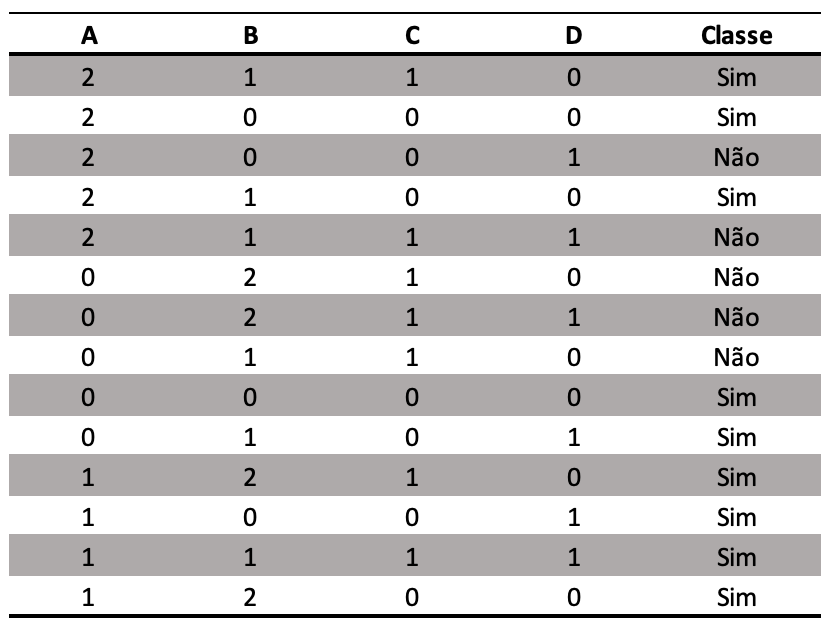
\includegraphics[width=8cm]{tab-5-2-3.png} 
  \end{figure}

\textit{Resposta:} 

\begin{figure}[H]
  \centering 
  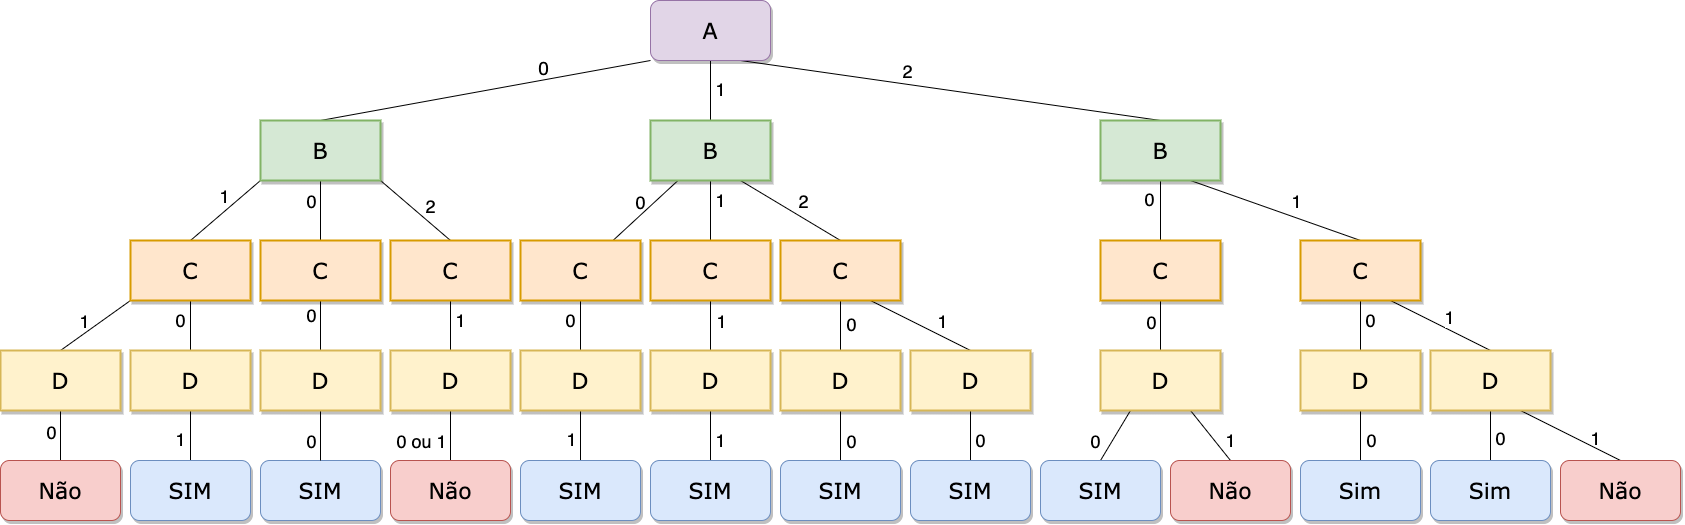
\includegraphics[width=17cm]{arvore-decisao.png} 
\end{figure}

\subsubsection{Aplique o classificador \textit{Naïve Bayes} na base de dados abaixo e determine o valor para classe \textbf{Jogar} dos seguintes objetos:}
\begin{enumerate}[label=\alph*]
    \item X = (Ensolarado, Branda, Alta, Não)
    \item Y = (Chuvoso, Fria, Alta, Sim)
    \item Z = (Ensolarado, Branda, Normal, Não)
    \item W = (Fechado , Fria, Normal, Sim)
\end{enumerate}

\begin{figure}[H]
    \centering 
    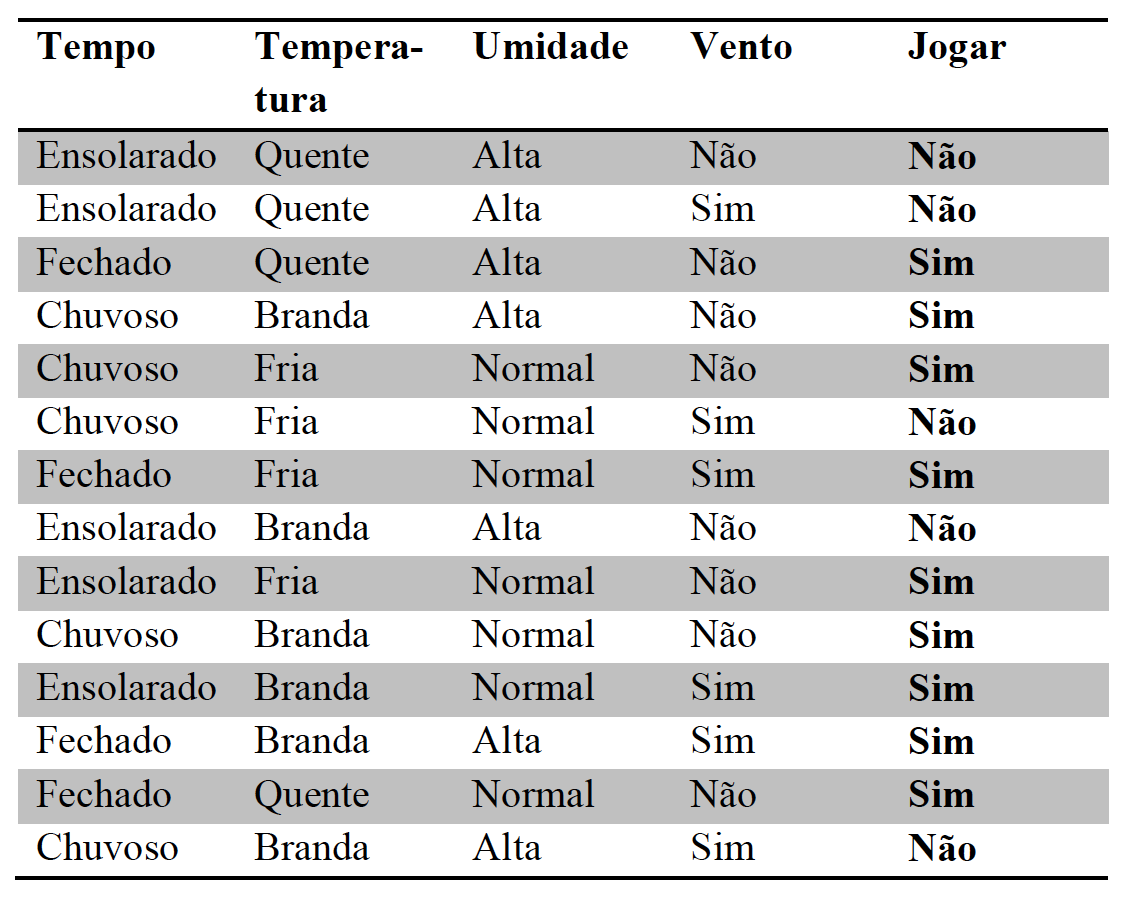
\includegraphics[width=8cm]{tab-5-2-4.png} 
  \end{figure}

\textit{Resposta:} 
\textbf{Teorema de Bayes:}
$P(C_i \mid x) = \dfrac{P(x \mid C_i)P(C_i)}{P(x)}$

\textbf{Probabilidade por atributo:}
  \begin{table}[H]
    \centering
    \begin{tabular}{cccc}
      \hline
      \rowcolor[HTML]{EFEFEF} 
      \multicolumn{1}{|c|}{\cellcolor[HTML]{EFEFEF}\textbf{Tempo}}       & \multicolumn{1}{c|}{\cellcolor[HTML]{EFEFEF}\textbf{Jogar = Sim}} & \multicolumn{1}{c|}{\cellcolor[HTML]{EFEFEF}\textbf{Jogar = Não}} & \multicolumn{1}{c|}{\cellcolor[HTML]{EFEFEF}\textbf{Total}} \\ \hline
      \multicolumn{1}{|c|}{Ensolarado}                                   & \multicolumn{1}{c|}{2/9 = 0.22}                                   & \multicolumn{1}{c|}{3/5 = 0.6}                                    & \multicolumn{1}{c|}{5/14 = 0.36}                            \\ \hline
      \multicolumn{1}{|c|}{Fechado}                                      & \multicolumn{1}{c|}{4/9 = 0.44}                                   & \multicolumn{1}{c|}{0/5 = 0}                                      & \multicolumn{1}{c|}{4/14 = 0.28}                            \\ \hline
      \multicolumn{1}{|c|}{Chuvoso}                                      & \multicolumn{1}{c|}{3/9 = 0.33}                                   & \multicolumn{1}{c|}{2/5 = 0.55}                                   & \multicolumn{1}{c|}{5/14 = 0.36}                            \\ \hline
      \multicolumn{1}{l}{}                                               & \multicolumn{1}{l}{}                                              & \multicolumn{1}{l}{}                                              & \multicolumn{1}{l}{}                                        \\ \hline
      \rowcolor[HTML]{EFEFEF} 
      \multicolumn{1}{|c|}{\cellcolor[HTML]{EFEFEF}\textbf{Temperatura}} & \multicolumn{1}{c|}{\cellcolor[HTML]{EFEFEF}\textbf{Jogar = Sim}} & \multicolumn{1}{c|}{\cellcolor[HTML]{EFEFEF}\textbf{Jogar = Não}} & \multicolumn{1}{c|}{\cellcolor[HTML]{EFEFEF}\textbf{Total}} \\ \hline
      \multicolumn{1}{|c|}{Quente}                                       & \multicolumn{1}{c|}{2/9 = 0.22}                                   & \multicolumn{1}{c|}{2/5 = 0.4}                                    & \multicolumn{1}{c|}{4/14 = 0.28}                            \\ \hline
      \multicolumn{1}{|c|}{Branda}                                       & \multicolumn{1}{c|}{4/9 = 0.44}                                   & \multicolumn{1}{c|}{2/5 = 0.4}                                    & \multicolumn{1}{c|}{6/14 = 0.43}                            \\ \hline
      \multicolumn{1}{|c|}{Fria}                                         & \multicolumn{1}{c|}{3/9 = 0.33}                                   & \multicolumn{1}{c|}{1/5 = 0.2}                                    & \multicolumn{1}{c|}{4/14 = 0.28}                            \\ \hline
      \multicolumn{1}{l}{}                                               & \multicolumn{1}{l}{}                                              & \multicolumn{1}{l}{}                                              & \multicolumn{1}{l}{}                                        \\ \hline
      \rowcolor[HTML]{EFEFEF} 
      \multicolumn{1}{|c|}{\cellcolor[HTML]{EFEFEF}\textbf{Umidade}}    & \multicolumn{1}{c|}{\cellcolor[HTML]{EFEFEF}\textbf{Jogar = Sim}} & \multicolumn{1}{c|}{\cellcolor[HTML]{EFEFEF}\textbf{Jogar = Não}} & \multicolumn{1}{c|}{\cellcolor[HTML]{EFEFEF}\textbf{Total}} \\ \hline
      \multicolumn{1}{|c|}{Alta}                                         & \multicolumn{1}{c|}{3/9 = 0.33}                                   & \multicolumn{1}{c|}{4/5 = 0.8}                                    & \multicolumn{1}{c|}{7/14 = 0.5}                             \\ \hline
      \multicolumn{1}{|c|}{Normal}                                       & \multicolumn{1}{c|}{6/9 = 0.67}                                   & \multicolumn{1}{c|}{1/5 = 0.2}                                    & \multicolumn{1}{c|}{7/15 = 0.5}                             \\ \hline
      \multicolumn{1}{l}{}                                               & \multicolumn{1}{l}{}                                              & \multicolumn{1}{l}{}                                              & \multicolumn{1}{l}{}                                        \\ \hline
      \rowcolor[HTML]{EFEFEF} 
      \multicolumn{1}{|c|}{\cellcolor[HTML]{EFEFEF}\textbf{Vento}}       & \multicolumn{1}{c|}{\cellcolor[HTML]{EFEFEF}\textbf{Joga = Sim}}  & \multicolumn{1}{c|}{\cellcolor[HTML]{EFEFEF}\textbf{Jogar = Não}} & \multicolumn{1}{c|}{\cellcolor[HTML]{EFEFEF}\textbf{Total}} \\ \hline
      \multicolumn{1}{|c|}{Sim}                                          & \multicolumn{1}{c|}{3/9 = 0.33}                                   & \multicolumn{1}{c|}{3/5 = 0.6}                                    & \multicolumn{1}{c|}{6/14 = 0.43}                            \\ \hline
      \multicolumn{1}{|c|}{Não}                                          & \multicolumn{1}{c|}{6/9 = 0.67}                                   & \multicolumn{1}{c|}{2/5 = 0.4}                                    & \multicolumn{1}{c|}{8/14 = 0.57}                            \\ \hline
    \end{tabular}
  \end{table}

  
  \begin{tabbing}
    \textbf{Probabilidade de Jogar (Sim/Não) $P(C)$:} 
    $P(Jogar=SIM) = \text{9/14} = 0.64$ \\
    $P(Jogar=NAO) = \text{5/14} = 0.36$ \\
  \end{tabbing}

  \textbf{\large Problema: a) - X = (Ensolarado, Branda, Alta, Não):}
  
  \begin{tabbing}
    \textbf{Probabilidade de Jogar=Sim por atributo:}\\
    $P(Tempo=Ensolarado \mid Jogar = Sim) =  0.22 $ \\
    $P(Temperatura=Branda \mid Jogar = Sim)  = 0.44 $ \\
    $P(Umidade=Alta \mid Jogar = Sim)  = 0.33 $ \\
    $P(Vento=Nao \mid Jogar = Sim) = 0.67 $ \\
    $P(Jogar=Sim) = 0.64$ \\
    $P(X \mid Jogar=Sim)P(Jogar=Sim) = 0.22 \cdot 0.44 \cdot 0.33 \cdot 0.67 \cdot 0.64 = 0.0137$ \\
  \end{tabbing}
  
  \begin{tabbing}
    \textbf{Probabilidade de Jogar=Nao por atributo:}\\
    $P(Tempo=Ensolarado \mid Jogar = Nao) =  0.6 $ \\
    $P(Temperatura=Branda \mid Jogar = Nao)  = 0.4 $ \\
    $P(Umidade=Alta \mid Jogar = Nao)  = 0.8 $ \\
    $P(Vento=Nao \mid Jogar = Nao) = 0.4 $ \\
    $P(Jogar=Nao) = 0.36$ \\
    $P(X \mid Jogar=Nao)P(Jogar=Nao) = 0.6 \cdot 0.4 \cdot 0.8 \cdot 0.4 \cdot 0.36 = 0.0276$ \\
  \end{tabbing}

  \begin{tabbing}
    \textbf{Probabilidade do total dos atributos:}\\
    $P(X) = P(Tempo=Ensolarado) \cdot P(Temperatura=Branda) \cdot P(Umidade=Alta) \cdot P(Vento=Nao)$ \\
    $P(X) = 0.36 \cdot 0.43 \cdot 0.5 \cdot 0.57$ \\
    $P(X) = 0.0441$  
  \end{tabbing}
  
  \begin{tabbing}
    \textbf{Probabilidade de Jogar:}\\
    $P(Jogar=Sim) \mid X) = \dfrac{0.0137}{0.0441} = 0.3106$ \\
    $P(Jogar=Nao) \mid X) = \dfrac{0.0276}{0.0441} = \textbf{0.6258}$
  \end{tabbing}

  \begin{tabbing}
    \textbf{Conclusão de X:}
    Probabilidade de Jogar = \textbf{NÃO}\\
  \end{tabbing}  

  \textbf{\large Problema: b) - Y = (Chuvoso, Fria, Alta, Sim):}
  
  \begin{tabbing}
    \textbf{Probabilidade de Jogar=Sim por atributo:}\\
    $P(Tempo=Chuvoso \mid Jogar = Sim) =  0.33 $ \\
    $P(Temperatura=Fria \mid Jogar = Sim)  = 0.33 $ \\
    $P(Umidade=Alta \mid Jogar = Sim)  = 0.33 $ \\
    $P(Vento=Sim \mid Jogar = Sim) = 0.33 $ \\
    $P(Jogar=Sim) = 0.64$ \\
    $P(Y \mid Jogar=Sim)P(Jogar=Sim) = 0.33 \cdot 0.33 \cdot 0.33 \cdot 0.33 \cdot 0.64 = 0.0076$ \\
  \end{tabbing}

  
  \begin{tabbing}
    \textbf{Probabilidade de Jogar=Nao por atributo:}\\
    $P(Tempo=Chuvoso \mid Jogar = Nao) =  0.6 $ \\
    $P(Temperatura=Fria \mid Jogar = Nao)  = 0.2 $ \\
    $P(Umidade=Alta \mid Jogar = Nao)  = 0.8 $ \\
    $P(Vento=Sim \mid Jogar = Nao) = 0.6 $ \\
    $P(Jogar=Nao) = 0.36$ \\
    $P(Y \mid Jogar=Nao)P(Jogar=Nao) = 0.6 \cdot 0.2 \cdot 0.8 \cdot 0.6 \cdot 0.36 = 0.0207$ \\
  \end{tabbing}

  
  \begin{tabbing}
    \textbf{Probabilidade do total dos atributos:}\\
    $P(Y) = P(Tempo=Chuvoso) \cdot P(Temperatura=Fria) \cdot P(Umidade=Alta) \cdot P(Vento=Sim)$ \\
    $P(Y) = 0.36 \cdot 0.28 \cdot 0.5 \cdot 0.43$ \\
    $P(Y) = 0.0217$  
  \end{tabbing}
  
  
  \begin{tabbing}
    \textbf{Probabilidade de Jogar:}\\
    $P(Jogar=Sim) \mid Y) = \dfrac{0.0076}{0.0217} = 0.3502$ \\
    $P(Jogar=Nao) \mid Y) = \dfrac{0.0207}{0.0217} = \textbf{0.9539}$
  \end{tabbing}

  \begin{tabbing}
    \textbf{Conclusão de Y:}
    Probabilidade de Jogar = \textbf{NÃO} \\
  \end{tabbing}

  \textbf{\large Problema: c) - Z = (Ensolarado, Branda, Normal, Não):}
  
  \begin{tabbing}
    \textbf{Probabilidade de Jogar=Sim por atributo:}\\
    $P(Tempo=Ensolarado \mid Jogar = Sim) =  0.22 $ \\
    $P(Temperatura=Branda \mid Jogar = Sim)  = 0.44 $ \\
    $P(Umidade=Normal \mid Jogar = Sim)  = 0.67 $ \\
    $P(Vento=Nao \mid Jogar = Sim) = 0.67 $ \\
    $P(Jogar=Sim) = 0.64$ \\
    $P(Z \mid Jogar=Sim)P(Jogar=Sim) = 0.22 \cdot 0.44 \cdot 0.67 \cdot 0.67 \cdot 0.64 = 0.0278$ \\
  \end{tabbing}

  \begin{tabbing}
    \textbf{Probabilidade de Jogar=Nao por atributo:}\\
    $P(Tempo=Ensolarado \mid Jogar = Nao) =  0.6 $ \\
    $P(Temperatura=Branda \mid Jogar = Nao)  = 0.4 $ \\
    $P(Umidade=Normal \mid Jogar = Nao)  = 0.2 $ \\
    $P(Vento=Nao \mid Jogar = Nao) = 0.4 $ \\
    $P(Jogar=Nao) = 0.36$ \\
    $P(Z \mid Jogar=Nao)P(Jogar=Nao) = 0.6 \cdot 0.4 \cdot 0.2 \cdot 0.4 \cdot 0.36 = 0.0069$ \\
  \end{tabbing}

  \begin{tabbing}
    \textbf{Probabilidade do total dos atributos:}\\
    $P(Z) = P(Tempo=Ensolarado) \cdot P(Temperatura=Branda) \cdot P(Umidade=Normal) \cdot P(Vento=Nao)$ \\
    $P(Z) = 0.36 \cdot 0.43 \cdot 0.5 \cdot 0.57$ \\
    $P(Z) = 0.0441$  
  \end{tabbing}
  
  \begin{tabbing}
    \textbf{Probabilidade de Jogar:}\\
    $P(Jogar=Sim) \mid Z) = \dfrac{0.0278}{0.0441} = \textbf{0.6303}$ \\
    $P(Jogar=Nao) \mid Z) = \dfrac{0.0069}{0.0441} = 0.1564$
  \end{tabbing}

  \begin{tabbing}
    \textbf{Conclusão de Z:}
    Probabilidade de Jogar = \textbf{SIM} \\
  \end{tabbing} 

  \textbf{\large Problema: d) - W = (Fechado, Fria, Normal, Sim):}
  
  \begin{tabbing}
    \textbf{Probabilidade de Jogar=Sim por atributo:}\\
    $P(Tempo=Fechado \mid Jogar = Sim) =  0.44 $ \\
    $P(Temperatura=Fria \mid Jogar = Sim)  = 0.33 $ \\
    $P(Umidade=Normal \mid Jogar = Sim)  = 0.67 $ \\
    $P(Vento=Sim \mid Jogar = Sim) = 0.33 $ \\
    $P(Jogar=Sim) = 0.64$ \\
    $P(W \mid Jogar=Sim)P(Jogar=Sim) = 0.44 \cdot 0.33 \cdot 0.67 \cdot 0.33 \cdot 0.64 = 0.0109$ \\
  \end{tabbing}

  \begin{tabbing}
    \textbf{Probabilidade de Jogar=Nao por atributo:}\\
    $P(Tempo=Fechado \mid Jogar = Nao) =  0 $ \\
    $P(Temperatura=Fria \mid Jogar = Nao)  = 0.33 $ \\
    $P(Umidade=Normal \mid Jogar = Nao)  = 0.2 $ \\
    $P(Vento=Sim \mid Jogar = Nao) = 0.6 $ \\
    $P(Jogar=Nao) = 0.36$ \\
    $P(W \mid Jogar=Nao)P(Jogar=Nao) = 0 \cdot 0.33 \cdot 0.2 \cdot 0.6 \cdot 0.36 = 0$ \\
  \end{tabbing}

  \begin{tabbing}
    \textbf{Probabilidade do total dos atributos:}\\
    $P(W) = P(Tempo=Fechado) \cdot P(Temperatura=Fria) \cdot P(Umidade=Normal) \cdot P(Vento=Sim)$ \\
    $P(W) = 0.28 \cdot 0.28 \cdot 0.5 \cdot 0.43$ \\
    $P(W) = 0.0168$  
  \end{tabbing}
  
  \begin{tabbing}
    \textbf{Probabilidade de Jogar:}\\
    $P(Jogar=Sim) \mid W) = \dfrac{0.0109}{0.0168} = \textbf{0.6488}$ \\
    $P(Jogar=Nao) \mid W) = \dfrac{0}{0.0168} = 0$
  \end{tabbing}

  \begin{tabbing}
    \textbf{Conclusão de W:}
    Probabilidade de Jogar = \textbf{SIM} \\
  \end{tabbing}

\end{document}